%%%%%%%%%%%%%%%%%%%%%%%%%%%%%%%%%%%%%%%%%%%%%%%%%%%%%%%%%%%%%%%%%%%%%%
% LaTeX Example: Project Report
%
% Source: http://www.howtotex.com
%
% Feel free to distribute this example, but please keep the referral
% to howtotex.com
% Date: March 2011 
% 
%%%%%%%%%%%%%%%%%%%%%%%%%%%%%%%%%%%%%%%%%%%%%%%%%%%%%%%%%%%%%%%%%%%%%%
% How to use writeLaTeX: 
%
% You edit the source code here on the left, and the preview on the
% right shows you the result within a few seconds.
%
% Bookmark this page and share the URL with your co-authors. They can
% edit at the same time!
%
% You can upload figures, bibliographies, custom classes and
% styles using the files menu.
%
% If you're new to LaTeX, the wikibook is a great place to start:
% http://en.wikibooks.org/wiki/LaTeX
%
%%%%%%%%%%%%%%%%%%%%%%%%%%%%%%%%%%%%%%%%%%%%%%%%%%%%%%%%%%%%%%%%%%%%%%
% Edit the title below to update the display in My Documents
%\title{Project Report}
%
%%% Preamble
\documentclass[paper=a4, fontsize=11pt]{scrartcl}
\usepackage[T1]{fontenc}
\usepackage{fourier}
\usepackage{subcaption}
\usepackage[english]{babel}					\usepackage{amsmath}										% English language/hyphenation
\usepackage[protrusion=true,expansion=true]{microtype}	
\usepackage{amsmath,amsfonts,amsthm} % Math packages
\usepackage[pdftex]{graphicx}	
\usepackage{import}
\usepackage{color}
\usepackage{url}
\usepackage{booktabs}
\usepackage{algorithm}
\usepackage[noend]{algpseudocode}
%%% Custom sectioning
\usepackage{sectsty}
\allsectionsfont{\centering \normalfont\scshape}


%%% Custom headers/footers (fancyhdr package)
\usepackage{fancyhdr}
\pagestyle{fancyplain}
\fancyhead{}											% No page header
\fancyfoot[L]{}											% Empty 
\fancyfoot[C]{}											% Empty
\fancyfoot[R]{\thepage}									% Pagenumbering
\renewcommand{\headrulewidth}{0pt}			% Remove header underlines
\renewcommand{\footrulewidth}{0pt}				% Remove footer underlines
\setlength{\headheight}{13.6pt}


%%% Equation and float numbering
\numberwithin{equation}{section}		% Equationnumbering: section.eq#
\numberwithin{figure}{section}			% Figurenumbering: section.fig#
\numberwithin{table}{section}				% Tablenumbering: section.tab#


%%% Maketitle metadata
\newcommand{\horrule}[1]{\rule{\linewidth}{#1}} 	% Horizontal rule

\title{
		%\vspace{-1in} 	
		\usefont{OT1}{bch}{b}{n}
		\normalfont \normalsize Department of Mathematics and Statistics, University of Otago  \\ [25pt]
		\horrule{0.5pt} \\[0.4cm]
		\huge Bayesian inference for process-based niche modelling \\
		\horrule{2pt} \\[0.5cm]
}
\author{
		\normalfont 								\normalsize
        Marnus Stoltz$^*$, David Bryant  \\[-3pt]		\normalsize
        \today
}
\date{}


%%% Begin document
\begin{document}
\maketitle
\section{Introduction}

The purpose of this report is to discuss Bayesian inference of the TTR-model. Another more ambitious goal is to outline an inference framework which can be used for models like the TTR. The report is structured as follow: In Section 1... we give a brief overview of the TTR model. Section 2 focuses on TTR model components in  . Thereafter in Section 2 we follow some general inference methods as described in \cite{GelmanBayesianAnalysis} in order to assess convergence and summarize the posterior densities of parameters of interest for the TTR model. In section ... we discuss inferences made from the Bayesian model analysis. [ And so on and so forth ...Will update this as structure of report becomes clearer]  

\subsection{The Thornley Transport resistance model}

The holy grail of plant ecology is understanding how physiological and morphological attributes of plants interact with environmental factors in order to define geographical distribution. Plant ecologists have considered  and debated these factors over the past century with a fierce intensity. Factors such as water, heat, light and soil are all thought to play a significant role. A prescient vision of how physiological and environmental factors shape plant distribution was laid down as early as 1902 by Schimper's Plant-geography on a physiological basis \cite{Schimper1902Plant-geographyBasis.} . 
The Thornley Transport Resistance model as implemented in \cite{Higgins2012APlants} is a model that upholds Schimper's vision. It models the uptake of carbon and nitrogen [see \cite{Dormann2012CorrelationDichotomy} for a version that includes phosphorous and \cite{Thornley1995Shoot:Models} for a version that includes water] and the transport of these substances from sources to sinks. The TTR-model relies on mechanistic plant growth and allocation in order to map the plant performance as a function of a small set of environmental covariates (often referred to as forcing variables). In turn this biomass mapping is then used as a basis for predicting the potential distribution of plants. 
The TTR-model will serve as a case study with the aim to illustrate useful mathematical and statistical techniques that can be employed in a more general ecological modeling setting. In particular we look at how an MCMC sampler \cite{Christen2010AT-walk} can provide insight into the predictive mechanisms of the TTR-model.

\subsubsection{Simple form of the TTR model}
Here we just give a brief description of the TTR model in it's simplest form. It's a set of 6 ordinary differential equations divided into two subsets that interact in order to model Biomass of a plant as shown in Figure 1.1. It's important to note that it's a deterministic system. This means that there is no randomness involved in the development of future states of the system. Therefore any given set of initial conditions with the same parameter values will always produce the same solution. We now state the governing ODE system for the simple TTR model. 
\begin{align}
	\frac{d M_s}{d t} = k_g \frac{C_s N_s}{M_s} - k_l \frac{M_s}{1 + \frac{K_M}{M_s}}  \\
    \frac{d C_s}{d t} = \frac{ M_s}{(1 + \frac{M_s}{K_A})(1 + \frac{C_s}{M_s J_C})} A - k_ck_g \frac{C_s N_s}{M_s} - \frac{M_s M_r}{M_s + M_r}(\frac{C_s}{M_s} - \frac{C_r}{M_r})\\
    \frac{d N_s}{d t} =\frac{M_s M_r}{M_s + M_r}(\frac{N_r}{M_r} - \frac{N_s}{M_s}) - k_N k_g \frac{C_s N_s}{M_s}
\end{align}
\begin{align}
	\frac{d M_r}{d t} = k_g \frac{C_r N_r}{M_r} - k_l \frac{M_r}{1 + \frac{K_M}{M_r}} \\
    \frac{d C_r}{d t} = \frac{M_s M_r}{M_s + M_r}(\frac{C_s}{M_s} - \frac{C_r}{M_r}) - k_c k_g \frac{C_r N_r}{M_r}\\
    \frac{d N_r}{d t} = \frac{M_r}{(1 + \frac{M_r}{K_A})(1 + \frac{N_r}{M_r J_N})} B - k_N k_g \frac{C_r N_r}{M_r} - \frac{M_s M_r}{M_s + M_r}(\frac{N_r}{M_r} - \frac{N_s}{M_s }) \label{ODE-TTR}
\end{align}
\begin{center}
\begin{figure}[h]
\centering
\input{TTR_diagram.pdf_tex}
 \label{TTRdiagram-poes}
 \caption{In the compartment model the compartments are divided into two process sets. Each set contains the same compartments but related to the physical structures namely the shoot and root as indicated using the subscripts. Each set consists of Biomass(M), Carbon (C) and Nitrogen (N). That is, $(M_s,C_s,N_s)$ for the shoot and $(M_r,C_r,N_r)$ for the root. The sets interact via transport between compartments of the same chemical element make-up and uptake of the chemicals are physiologically determined and the rate of uptake are determined by the mass of the structure}
\end{figure}
	\end{center}

\subsubsection{TTR model with environmental forcing factors}

Mathematically adding environmental variables changes constants into functions of time. We now proceed to state these functions for the TTR model as defined and physiologically justified in \cite{Higgins2012APlants}.   
\begin{align}
A(t) = A\min\left[ \bar{E} \circ Tmax(t),E \circ W(t), E \circ N_r(t), E \circ R_(t) \right] \\
B(t) = B\min\left[ \bar{E} \circ T(t), E \circ W(t), E \circ N(t)\right] \\
k_g(t) = k_g\bar{E} \circ F(t) \\
k_l(t) = k_l E \circ G(t) \label{TTR forcing functions}
\end{align}
In order to introduce this environmental dependence for the TTR model we change the following constants, $A$, $B$, $k_g$, $k_l$ into functions of time, i.e ($A(t)$, $B(t)$, $k_g(t)$, $k_l(t)$) as shown by \ref{TTR forcing functions}. The constants dictate the upper bounds for biomass growth and -loss.  The environmental forcing factors added are minimum temperature ($T_{min}$), mean temperature ($T_{mean}$), maximum temperature ($T_{max}$), soil water availability ($W$), soil radiation ($R$) nitrogen content $(N)$ of the soil and Nitrogen content in the roots ($N_r$). The environmental forcing factors are biomass growth inhibitors except for $k_l(t)$ where $(T_min)$ is a biomass loss inhibitor. The above described growth and loss inhibition is clear from the way the evaluation functions are defined in \ref{Evaluation Functions}.   
Normalized environmental factors are fed into the specified evaluation function in order to obtain an inhibition value between [0,1]. The environmental factor that contributes the most inhibition (i.e lowest inhibition value) are used to represent inhibition of growth or loss at time $t$ for a specific function. The general shape of the linear evaluation functions are shown in \ref{evaluation function graphs}. In a following section we will consider these evaluation functions in more detail and whether smoothing of these functions would be beneficial for niche projections of plant species.   
\begin{align}
  E(x)=\begin{cases}
  \dfrac{x - \beta_1}{\beta_2 - \beta_1},& \beta_1 < x < \beta_2 \\
  0, & \text{otherwise} \\
  \end{cases} \\ 
  \bar{E}(x)=\begin{cases}
  \dfrac{x - \bar{\beta_1}}{\bar{\beta_2} - \bar{\beta_1}} , & \bar{\beta_1} < x < \bar{\beta_2} \\
  1, & \bar{\beta_2} < x < \bar{\beta_3} \\
  \dfrac{\bar{\beta}_4 - x}{\bar{\beta}_4 - \bar{\beta}_3},   & \bar{\beta}_3 < x < \bar{\beta}_4 \\
  0, & \text{otherwise}  \label{Evaluation Functions} \\
        \end{cases}        
\end{align}

\begin{figure}[h]
\begin{subfigure}{.5\textwidth}
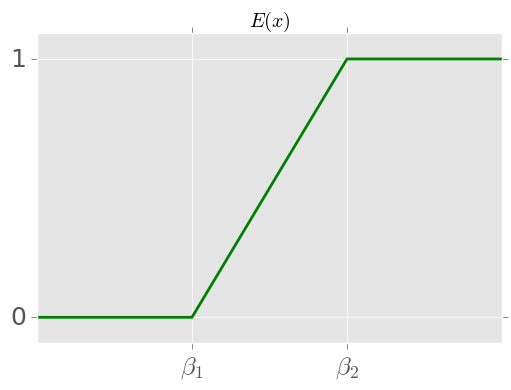
\includegraphics[scale=0.5]{E.png}
\end{subfigure}
\begin{subfigure}{.5\textwidth}
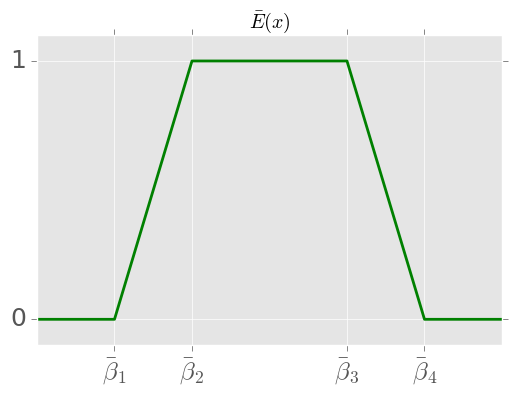
\includegraphics[scale=0.5]{E_.png}
\end{subfigure}
\caption{In this figure we illustrate the general shape of the linear evaluation functions as described in \ref{Evaluation Functions}. $E(x)$ is an increasing function from $[0,1]$ while $\bar{E}(x)$ has a trapezoidal shape with maximum value of 1.} 
\label{evaluation function graphs}
\end{figure}


\newpage
\begin{figure}[h]
\centering
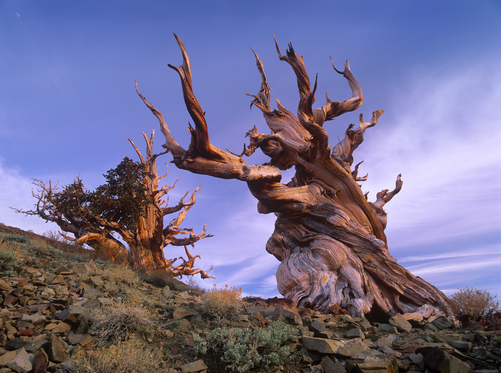
\includegraphics[scale=2]{bristlecone-pine-1.jpg}
\caption{Pinus aristata, the Rocky Mountain bristlecone pine, is a species of pine native to the United States. It appears in the Rocky Mountains in Colorado and northern New Mexico, with isolated populations in the San Francisco Peaks in Arizona and the Kaibab National Forest north of the Grand Canyon. \cite{2006Growth-FormReport} gives an  in-depth description of the species growth-form characteristics.} 
\label{pinus aristata}
\end{figure}

\section{A closer look at the model components}

In this section we investigate the components of the model. In order to achieve this we'll study the TTR-model via an example. We use environmental data on a single conifer species in order to investigate growth and inhibition predictions of the model. The species used in the case study is known as Pinus Aristata, see Figure \ref{pinus aristata}. 

The goal is to get a better understanding of the workings of the components of the TTR model. The initial conditions, Table \ref{initial-conditions}, and model parameters, Table \ref{fixed-parameters} stated are the same as used in \cite{Higgins2012APlants}. 

We assume that our model is already optimized and restrict ourselves to the evaluation process and function construction. The beta parameters used are stated in Table ...\ref{}. We remind the reader that a comprehensive description of beta parameter distributions and optimization are discussed in Section ...\ref{} that follow. 

The data for the environmental forcing variables are available at \cite{DatabaseAristata}. It consists of a set of 107 distinct geographical locations each with a set of 5 environmental forcing factors namely, maximum temperature, minimum temperature, mean temperature, soil water content and soil nitrogen content. Each environmental forcing factor consists of 12 measurements. Each measurement are interpreted as a monthly indicator for a specific environmental factor of a geographic location. Except for the soil nitrogen content $(N)$ which is assumed to be a constant measure for each location. In order to give a detailed account of the model we look at location 33 with normalized environmental measures as stated in Table \ref{loc-33-data}. 


Now that we've stated and described all the required data to make a biomass prediction we shift our focus back to the TTR-model and the growth dynamics. In order to numerically integrate the TTR model with environmental forcing factors as described by the set of ordinary differential equations \ref{ODE-TTR} with time-dependent functions \ref{TTR forcing functions} we apply a numerical method known as the Runga-Kutta method \cite{HAIRER2000Solving1}. This method is reasonably simple and robust and is a good general candidate for numerical solution of differential equations. An assumed equilibrium of an approximated solution is only reached after 600 time steps (months) as seen in Fig \ref{loc-33-growth}.  It is also important to note that for these timesteps the model cycles through the environmental data. That is to say that we assume that environmental conditions remain consistent for consecutive years. We see in Figure \ref{evaluation-explain} the role evaluation functions,\ref{Evaluation Functions} play in \ref{TTR forcing functions} and the contribution it makes towards growth prediction. 



For the sake of brevity we just looked at one forcing function $B(t)$ that is related to nitrogen in the root. In Figure \ref{evaluation-explain} (a), (b) \& (c) we see evaluations of the normalized data. In \ref{evaluation-explain} (d) we see a timeplot of these values. Lastly in Figure \ref{evaluation-explain} we see the lowerbound of the combined timeseries plot. This piecewise contructed function is then used as the inhibition of nitrogen in the root when solving the system \ref{ODE-TTR}, \ref{TTR forcing functions}. Note that the process is exactly the same for the other time-dependent functions. Approximated solutions for the system \ref{ODE-TTR}, \ref{TTR forcing functions} of typical growth and lack of growth are given in Figures \ref{loc-33},\ref{loc-54}. In Figure \ref{loc-33} we show the approximated solution of the TTR-model with initial conditions, Table \ref{initial-conditions}, model parameters, Table \ref{fixed-parameters} and data, Table \ref{loc-33-data}. Again for the sake of brevity we do not include the data table used for location 54 as shown in Figure \ref{loc-54}. 

To get a better understanding of the optimization of the model we provide a logscale histrogram plot \ref{evaluations-histogram}. This histogram plot summarizes the evaluation values for all the environmental variables off all the time-dependent functions over all 107 locations. We see that there's at least 2 orders of magnitude difference in the frequency that the functions are evaluated at $x = 0$, $ x = 1$ vs. $x \in (0,1)$. 
\vspace{1cm}
\begin{table}
\begin{center}
\begin{tabular}{|c c c c c c c c c c|}
\multicolumn{10}{|c|}{Fixed parameters} \\
 $A_0$ & $B_0$ & $J_c$ & $J_N$ & $K_A$ & $K_m$ & $k_l$ & $k_c$ & $k_n$  & $k_g$    \\ 
 0.1 & 0.02 & 0.1 & 0.01 & 3 & 1.5 & 0.1 & 0.5 & 0.025 & 20
\end{tabular}
\caption{ These fixed parameters are the upperbounds for growth  and loss therefore it remains fixed across all locations}
\label{fixed-parameters}
\end{center}
\end{table}
\vspace{-1cm}
\begin{table}]
\begin{center}
\begin{tabular}{|c c c c c c|}
\multicolumn{6}{|c|}{Initial conditions} \\
 $M_s$ & $C_s$ & $N_s$ & $M_r$ & $C_r$ & $N_r$ \\ 
 0.1 & 0.005 & 0.001 & 0.1 & 0.005 & 0.001  
\end{tabular}
\caption{ The initial conditions can be interpreted as an opportunity to grow at a geographical location therefore this will also remain constant for all locations}
\label{initial-conditions}
\end{center}
\end{table}

\begin{figure}[ht]
\begin{subfigure}{.33\textwidth}
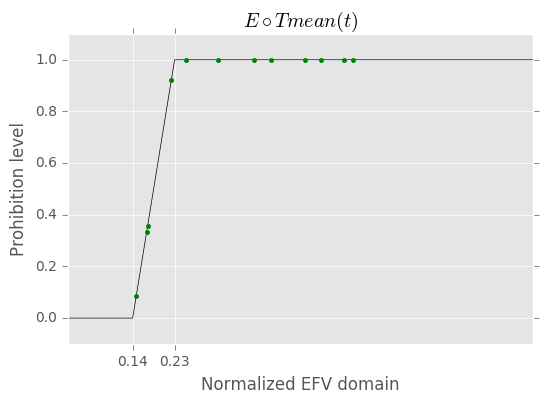
\includegraphics[scale=0.33]{E_Tm.png}
\caption{}
\label{E_Tm}
\end{subfigure}
\begin{subfigure}{.33\textwidth}
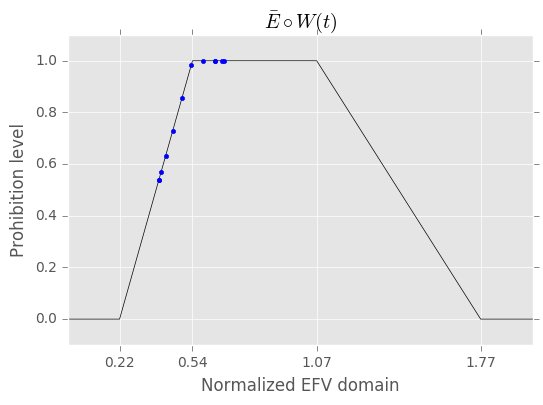
\includegraphics[scale=0.33]{E_W.png}
\caption{}
\label{E_W}
\end{subfigure}
\begin{subfigure}{.33\textwidth}
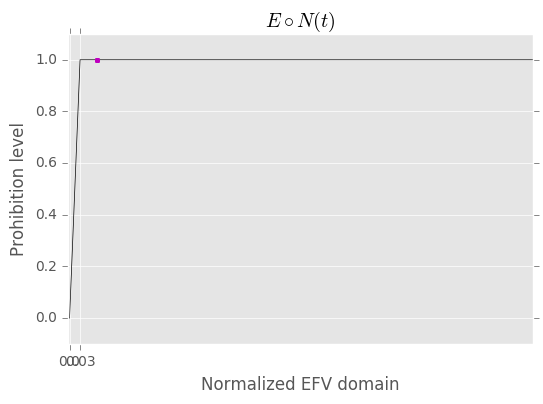
\includegraphics[scale=0.33]{E_N.png}
\caption{}
\label{E_N}
\end{subfigure}
\begin{subfigure}{.5\textwidth}
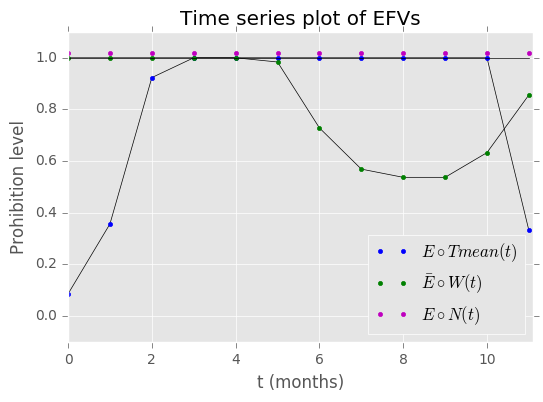
\includegraphics[scale=0.5]{timeseries_NWT.png}
\caption{Timeseries plots of Fig \ref{evaluation-explain} (a),(b) \& (c) }
\label{timeseries_NWT}
\end{subfigure}
\begin{subfigure}{.5\textwidth}
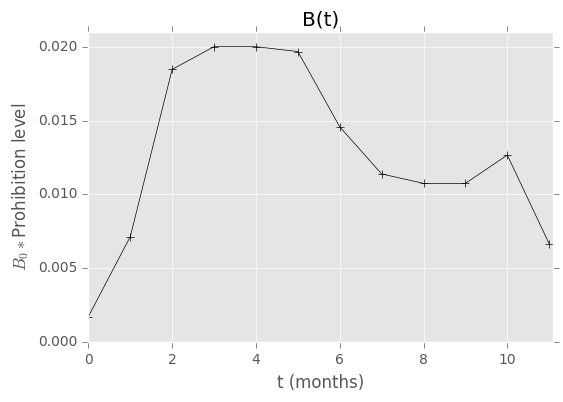
\includegraphics[scale=0.5]{B_t.png}
\caption{B(t) or lowerbound of timeseries plot.}
\label{B_t}
\end{subfigure}
\caption{ Note that $B_0$ is added as a constant}
\label{evaluation-explain}
\end{figure}

\begin{figure}[ht]
\centering
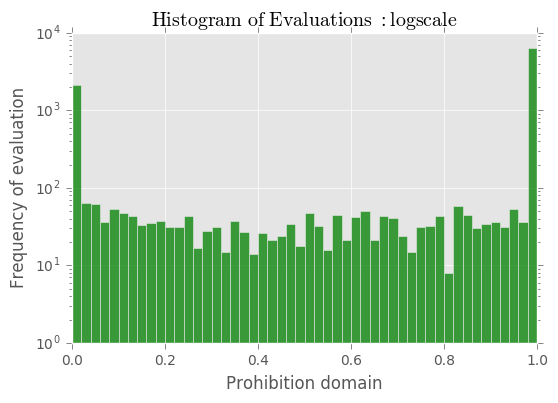
\includegraphics[scale=0.65]{histo_EP.png}
\caption{} 
\label{evaluations-histogram}
\end{figure}

\begin{figure}[ht]
\begin{subfigure}{.5\textwidth}
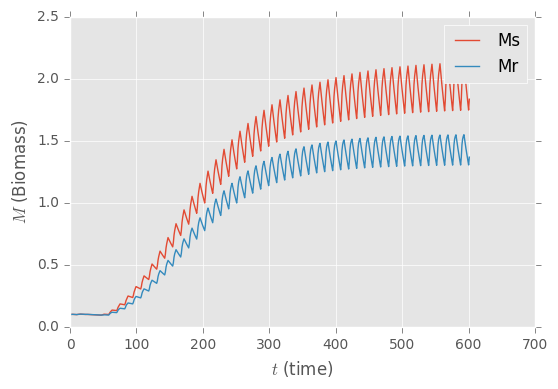
\includegraphics[scale=0.5]{growth.png}
\caption{Growth prediction for location 33.}
\label{loc-33-growth}
\end{subfigure}
\begin{subfigure}{.5\textwidth}
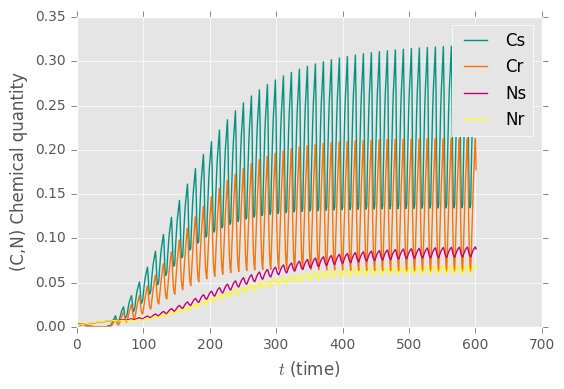
\includegraphics[scale=0.5]{loc-33-cc.png}
\caption{Chemical components for location 33}
\label{loc-33-cc}
\end{subfigure}
\begin{subfigure}{.5\textwidth}
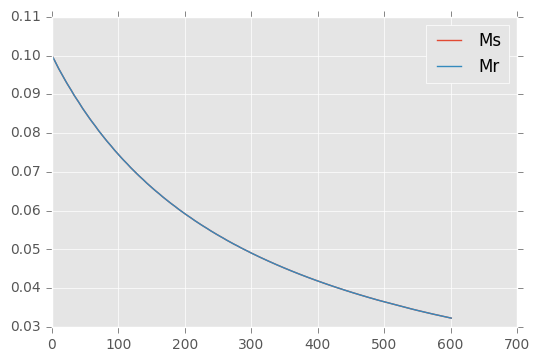
\includegraphics[scale=0.5]{inhibition.png}
\caption{Growth prediction for location 54.}
\label{loc-54-growth}
\end{subfigure}
\begin{subfigure}{.5\textwidth}
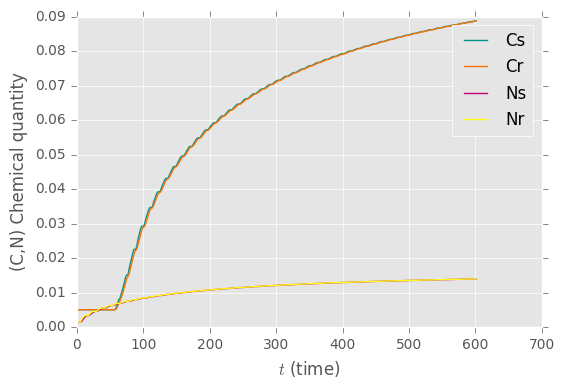
\includegraphics[scale=0.5]{loc-54-cc.png}
\caption{Chemical components for location 54. }
\label{loc-54-cc}
\end{subfigure}
\caption{Here we observe typical behavior of the model when it predicts growth and failure of growth.}
\label{loc-54}
\end{figure}


\section{Bayesian Inference of the TTR model}
The importance of conducting Bayesian analysis on any predictive model cannot be overstated. It plays a very important role when we want to check model assumptions. In order to stake a claim on the models predictive capabilities it is first necessary to lay a firm foundation for the model. This foundation can then be used to justify model parameters and assumptions.  [Will have to find some smart guys take on the importance of Bayesian analysis in this context and add as reference]

In this section our goal is to provide a summary of the Bayesian inference conducted on the TTR model. Technical details of the methods employed will mostly just be referenced or briefly described as this is not the current focus. Our primary task in this section is to use the Bayesian framework to summarize  $p(\beta|data)$, the posterior distribution of the beta parameters given a set of data for the TTR model. Due to the complexity of the model $p(\beta|data)$ cannot be directly calculated and we resort to employing a commonly used MCMC method. This MCMC algorithm is discussed in the first section. We briefly highlight why this algorithm is convenient for usage in these types of investigations and describe the link between the MCMC algorithm and the TTR model. We then move on to describing debugging methods using the t-walk. Thereafter we concern ourselves with the convergence of Markov chains. Once this is established we give a brief summary of the parameter inference. [Will insert further structure description once section is refined/complete]   

\subsection{T-walking - Our preferred mode of transport/ MCMC weapon of choice}
Here we give a short motivation for our MCMC algorithm of choice, the t-walk. The t-walk is a scale-independent, adaptive MCMC algorithm for arbitrary continuous distributions and correltation structures. 
It is often the case that non-specialists get stuck on the details of algorithm design instead of focusing on the task at hand. Whether it is verifying current model parameters, exploring possible parameter extensions/reductions or summarizing parameter behaviour. All of these tasks are lengthy and arduous processes. It is therefore convenient to have an MCMC algorithm in ones analysis toolbox that works straight out of the afore mentioned toolbox. As stated in \cite{Christen2010AT-walk} the t-walk results in "a simple, mathematically tractable algorithm that lends itself to use as a black-box sampler, since only evaluation of the objective function (likelihood function) is needed; there being no need to calculate any conditional distributions, etc. nor some prior knowledge of the number of modes, tails etc.". 
It is worth mentioning to the reader that the sampler performed satisfactorily in multiple examples, shown in \cite{Christen2010AT-walk}, considering dimensions from 2 to 200. Therefore it is usable for a broad range of problems and worth keeping in mind for future work.
The t-walk is available as an R (R Development Core Team 2008) and Python http://www.python.org/ packages (and is also available in MatLab and C++) at http://www.cimat.mx/~jac/twalk/ and will soon be included in the PyMC package at http://code.google.com/p/pymc/. [still have to add the links as references]

\subsubsection{Likelihood function of the TTR model}
In order to sample from the posterior distribution using the t-walk the only required input is the likelihood function $p($data$|\beta)$ of the TTR model. In this section we simply state how $p(data|\beta)$ is calculated without explaining the role of the likelihood function in context of an MCMC sampler. In order to gain a better understanding of this we refer the reader to \cite{GelmanBayesianAnalysis} for a detailed account. In the TTR model $p(data|\beta)$ is calculated as follow. The first step is to change our biomass predictions into probabilities. Recall that $M_i$ is the biomass prediction for a specific location $i$. The probability of observing the plant species at location i is calculated in \cite{Higgins2012APlants} as follow, 
\begin{equation}
p_i = 1 - e^{-M_i} \text{, for $i = 1,...,N$}
\label{prob of M}
\end{equation}  
The probability vector that follows from \ref{prob of M} is used together with the given absence presence data to calculate the likelihood function \ref{likelihood}. We remind the reader that the absence presence data is just a set of binary indications(0 or 1) of whether a species was observed at a given site $i$.   
\begin{equation}
p(data|\beta) = \log(\prod_{i \in A}p_i\prod_{i \in B}(1-p_i))
\label{likelihood}
\end{equation}  
where we define the following two mutually exclusive sets, 
$A$ is the set of locations of the given data where the species is present.
$B$ is the set of locations of the given data where the species is absent.
The selection process for set B, that is to say which sites we should include as absence sites is a point of contention in the literature [add references] and we will dedicate a section
to describe the underlying issues and possible solutions that have been employed to deal with the problem. For now we
just assume that B is a given set of absence points.

\subsection{Using the t-walk as a debugging tool}
In this section we discuss debugging the model in order to make sure that our parameter inferences are reliable. We employed two methods for debugging the model. First we have to debug the debugger. The first method ensures that our MCMC algorithm is sampling properly. This is achieved by setting the loglikelihood function $p(data|\beta) = 1$, $\forall \beta$. Simply put we assume equivalence for all possible move suggestions. Thus any $\beta$ will describe the data equally "well". Therefore if the MCMC is working properly we should observe a uniform distribution over the parameter domain.  We see in Figure \ref{fig:mcmc_debug_uni_dist} that the MCMC indeed seems to be doing exactly that after implementing this method.  Uniformly distributed scatterplots are observed over the reasonable parameter domain. 
We define reasonable parameters in our case as parameters that fall within the predetermined parameter domain, that is $ 0 <\beta_i < 2$  $\forall i$, and the obvious model restrictions. That is,  for $E(x)$ we have $0 <\beta_1 < \beta_2 < 2$ and $\bar{E}(x)$ we have $\beta_{i} < \beta_{i+1}$ for $i = 1,2,3$.
\begin{figure}[ht]
\centering
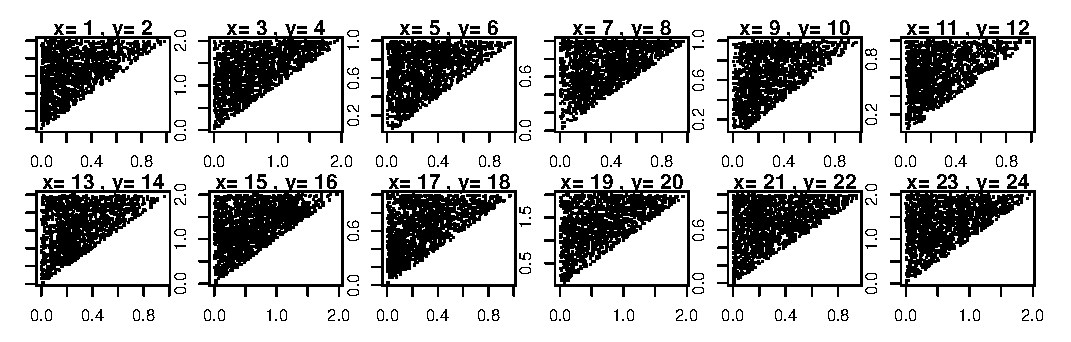
\includegraphics[scale=0.8]{mcmc_debug.eps}
\caption{We observe uniformly distributed scatterplots of the reasonable domain for the $\beta$ parameters.} 
\label{fig:mcmc_debug_uni_dist}
\end{figure}

It is clear that should uniformity fail to be observed then we need to pay attention to our MCMC algorithm first. Therefore isolating any possible problems.
Now once it has been established that the MCMC is doing what it should be doing we can move on to employing the second test. The second test consists of generating some fake data by using reasonable parameters then fitting the model using the fake data to see if we get can get the same parameters out again. The problem here is how do we know we have reasonable parameters if we don't know that the model is working. A possible solution is to obtain crude estimates using a different method for model fitting. Should the parameters not correspond more or less than the model might be faulty. The other possibility could be that the data might have more than one peak where optimality can be achieved. This is why it is necessary to provide a summary of the parameter distributions. It is unclear whether the fake data test is actually useful. Nonetheless we shall give a short algorithm for generating fake data for the TTR model. The procedure for generating fake data is described by Algorithm \ref{alg:generate_fake_data}.

\begin{algorithm}
\caption{Generate fake data for debugging purposes}\label{alg:generate_fake_data}
\begin{algorithmic}[1]
\Procedure{Generate}{$p_{\alpha}$}\Comment{$p_{\alpha}$ is the site probabilities}
\State $p_{\beta} \gets \textit{$n$ random numbers between 0 and 1} $
\State $s \gets \textit{zero vector of size $n$}$
\For{$i=1:n$}
\If{$p_{\alpha}(i) > p_{\beta}(i)$} \Comment{Species is present at a location if this holds}
\State $s(i) \gets 1$ 
\EndIf
\EndFor
\State \textbf{return} $s$
\EndProcedure
\end{algorithmic}
\end{algorithm}

Also, an  issue that needs to be discussed in further detail: Should a debugging test fail how can we isolate the problem.  A good debugging test will have no ambiguity in terms of where the error might be. Can we use the two aforementioned tests as good example of a debugging test and a not so good example. Maybe expand this section by adding more examples of tests?  

\subsection{Approximate convergence of the beta parameter Markov chains}
We now assume that our model is debugged and has no obvious flaws. Therefore we can start sampling from the posterior distribution of the TTR model using the t-walk. In order to ensure that our initial conditions (starting points for the sampler) are overdispersed we ran the sampler with four different sets of upper and lower bound combinations over the reasonable parameter domain.
The sampler ran for a million iterations per set of initial conditions therefore producing 4 Markov chains of a million values each per parameter. The rule of thumb is to burn half of the chain.  In this section we are interested in whether these Markov chains of the beta parameters using the t-walk converge. [Probably have to define convergence in this context] It is clear that without having established approximate convergence the inferences are meaningless.  In order to assess the convergence of the chains we apply the Gelman-Rubin convergence diagnostics [reference]. In a nutshell Gelman-Rubin convergence diagnostics calculates variance in a chain and between the chains and then takes a ratio of these values to give an indication of convergence. 
We use the "coda" [reference] package in R to achieve this. The documentation states that the 'potential scale reduction factor' is calculated for each variable in x, together with upper and lower confidence limits. Approximate convergence of the Markov chain seems to be achieved when the upper limit is close to 1. 
The details of the Gelman-Rubin convergence calculations are stated in \cite{GelmanBayesianAnalysis}. We see that the point estimators in Table \ref{Gelman-Rubin convergence table} varies from close to 1 to not close enough?. A potential problem with calculating the Gelman-Rubin shrink factor   at a point is that there's no indication of convergence. The shrink factor might be close to 1 by chance. By calculating the shrink factor at several points in time, as seen in Figure \ref{Gelman-Rubin convergence plot} we can confirm whether the shrink factor has really converged, or whether it is fluctuating. Our preference of this method for monitoring convergence is because our lack of enthusiasm to analyze time-series graphs of Markov chains. As stated in \cite{GelmanBayesianAnalysis} "Inspection of such plots is a notoriously unreliable method of assessing convergence and in addition is unwieldy when monitoring a large number of quantities of interest..."  .[Not sure if I should include Figure 3.2, maybe add it into an appendix, that way I can add the graphs for all 24 parameters?]
\begin{table}
\begin{center}
\begin{tabular}{c c c | c c c | c c c | }
 \toprule
 $\beta_i$ & Point est. & Upper C.I. &  $\beta_i$ & Point est. & Upper C.I. &   $\beta_i$ & Point est. & Upper C.I.  \\ 
 \midrule
  1 & 1.21 & 1.51 & 2 & 1.23 & 1.53 & 3 & 1.05 & 1.13 \\
  4 & 1.10 & 1.23 & 5 & 1.61 & 2.47 & 6 & 1.40 & 1.87 \\
  7 & 1.28 & 1.68 & 8 & 1.07 & 1.18 & 9 & 1.55 & 2.59 \\
  10 & 1.36 & 1.82 & 11 & 1.46 & 2.17 & 12 & 1.62 & 2.47 \\
  13 & 1.08 & 1.19 & 14 & 1.10 & 1.24 & 15 & 1.22 & 1.53 \\
  16 & 1.06 & 1.13 & 17 & 1.39 & 1.91 & 18 & 1.33 & 1.72 \\
  19 & 1.07 & 1.11 & 20 & 1.20 & 1.52 & 21 & 1.06 & 1.14 \\
  22 & 1.06 & 1.14 & 23 & 1.04 & 1.08 & 24 & 1.11 & 1.27 \\
 \bottomrule
\end{tabular}
\end{center}
\caption{}
\label{Gelman-Rubin convergence table}
\end{table}
\subsection{Graphical inference summary of the beta parameters}
Now that we have established approximate convergence of our Markov chains we can summarize our findings. Note that the slang in the Bayesian world for this a well mixed chain. This statement leads us to hastily plot the results in a summary. This however can first be tidied up by only using the independent draws from the Markov chains. In a more formal tone we calculate the effective sample size. This calculation stems from the Gelman-Rubin calculations since we use a ratio of the variance between the chains and the variance in the chains multiplied by the number of iterations and number of Markov chains. All this mathematical splendour can be found in \cite{GelmanBayesianAnalysis} [page 296 - 298]. 

After doing this calculation we find that our effective sample size is around a 1000 for each parameter. Given this estimate in order to get an independent sample one has to use at least every 500th value in our combined Markov chain. We note that since we don't need a thousand independent draws we only took every 5000th value. The above correction indicates that we can use the effective sample size to figure out for how long we should be running our sampler in order to get a decent inference of the parameters. It's clear from this example that should we repeat this exercise we can significantly reduce the number of iterations. This will obviously improve the computational time for our modeling problem. In Figure \ref{fig: parameter summary} we provide a parameter inference summary for which we applied the the afore mentioned procedure. 

Lastly, it is important to quantify uncertainty around point estimators in order to verify their validity. In the next section we will attempt to outline a procedure to use our Bayesian framework along side other optimization methods.

\section{Using an MCMC algorithm for optimization purposes}
Still have to think about what to include in this section

\chapter{Fischer-Wright diffusion in 1D}
\section{Brief overview}
The aim is to find an efficient method to evaluate the Kolmogorov forward equation for the Fischer-Wright diffusion operator.
We state the Fischer-Wright diffusion operator
\begin{equation}
 Lu = a(x)\frac{d^2u}{dx^2} + b(x)\frac{du}{dx} \label{FW-operator}
\end{equation}
where a(x),b(x) $\in C^\infty([0,1])$. We assume that a(x)=x(1-x) remains fixed but $b(x) = \gamma x(1-x) + \xi_1 (1-x) - \xi_2 x$ will vary depending on the parameters $(\gamma, \xi_1, \xi_2)$. $a(x)$ is referred to as the infinitesimal mean and $b(x)$ the infinitesimal variance. The parameters govern the mutation and survival rates of an allele.
We are interested in the Kolomogorov backward equation with zero flux boundary conditions. This require us to derive the adjoint operator as shown below. We remind the reader that the adjoint operator $L^*$ is defined in terms of an inner product $<\dot,\dot>$ as follow $<Lu,v> = <u,L^*v>$.

\begin{eqnarray}    
<Lu,v> & = <a(x)u' + b(x)u, v> 
\end{eqnarray}

\begin{eqnarray*}    
 <Lu,v> = <a(x)u" + b(x)u', v> \\
        = <u", a(x)v > + <u', b(x)v> \\
		= -<u', (a(x)v)'> + a(x)u'v|^1_0 - <u, (b(x)v)'> + b(x)uv|^1_0 \text{ I.B.P} \\
		= <u, (a(x)v)"> - u(a(x)v)'|^1_0 + a(x)u'v|^1_0 - <u, (b(x)v)'> - b(x)uv|^1_0 \text{ I.B.P} \\
        = <u, (a(x)v)"> - u(a(x)v)'|^1_0 + a(x)u'v|^1_0 - <u, (b(x)v)'> - b(x)uv|^1_0 \text{ notice that $a(0)=a(1)=0$} \\
        = <u, ((a(x)v)'-(b(x)v)')'>  + (a(x)u'- b(x)u)v|^1_0 
\end{eqnarray*}

It is clear from the above derivation that in order for $L^*v = ((a(x)v)'-(b(x)v)')'$ to be the adjoint operator we need to impose the following boundary condition $a(x)u'- b(x)u = 0$ for $x=0,1$. These boundary conditions are known as the "zero flux" boundary conditions. We can now state the Kolmogorov forward equation, the equation of interest, for the Fischer-Wirght diffusion is defined as $\frac{du}{dt} - L^*u = 0$.

\section{Problem statement}
A rough sketch of the problem that we seek to compute efficiently is given as follow.

Suppose u(x,t) satisfies,
\begin{eqnarray*}
L^*u = 0\\
u(x,0) = \delta(x-x_0)\\
(a(x)u'- b(x)u) = 0 \text{ for } x\in[0,1], \forall t
\end{eqnarray*} 
Now our process as seen in Figure can be described as $\int_0^1u (x,\tau)g(x)dx = <u(x,\tau), g(x)\delta(t - \tau)>= h(\tau)/h(x_0,\tau)$. We want to know what is $\frac{dh}{d\tau}$. This we can see from previous calculations that,
$\frac{dh}{d\tau} = \int\frac{d}{dx}(a(x)\frac{du(x,\tau)}{dx} - b(x))g(x)$

The rate of change with respect to time is given in terms of change with respect to probability distribution. Therefore without any change in space did time really pass?

\newpage
\bibliographystyle{unsrt}
\bibliography{Mendeley}

\begin{figure}[ht]
\begin{subfigure}{.5\textwidth}
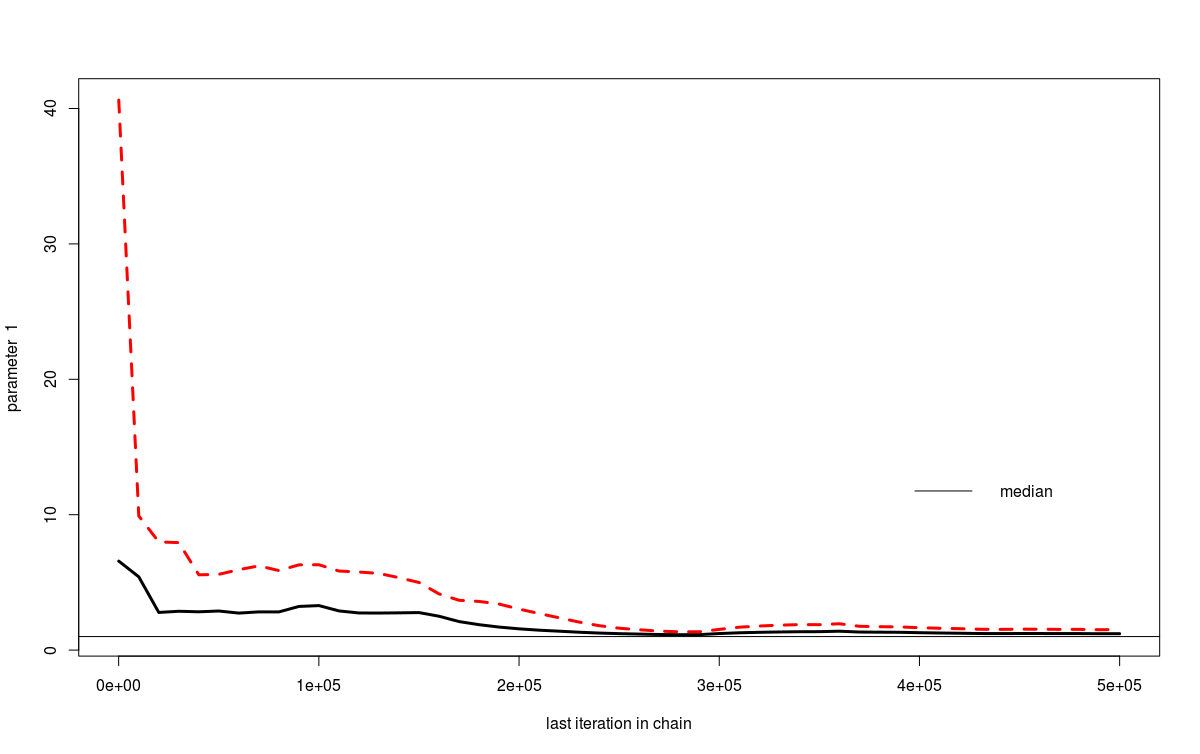
\includegraphics[scale=0.2]{scale_red_par1.png}
\caption{}
\label{}
\end{subfigure}
\begin{subfigure}{.5\textwidth}
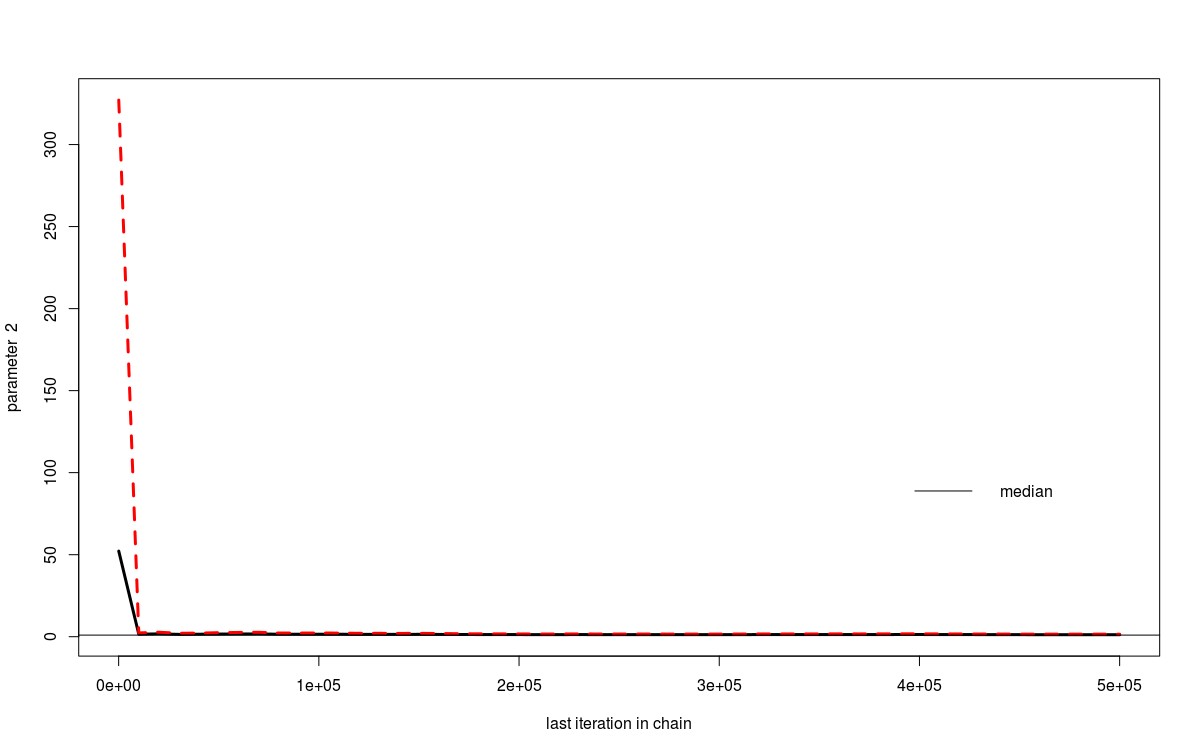
\includegraphics[scale=0.2]{scale_red_par2.png}
\caption{}
\label{}
\end{subfigure}
\begin{subfigure}{.5\textwidth}
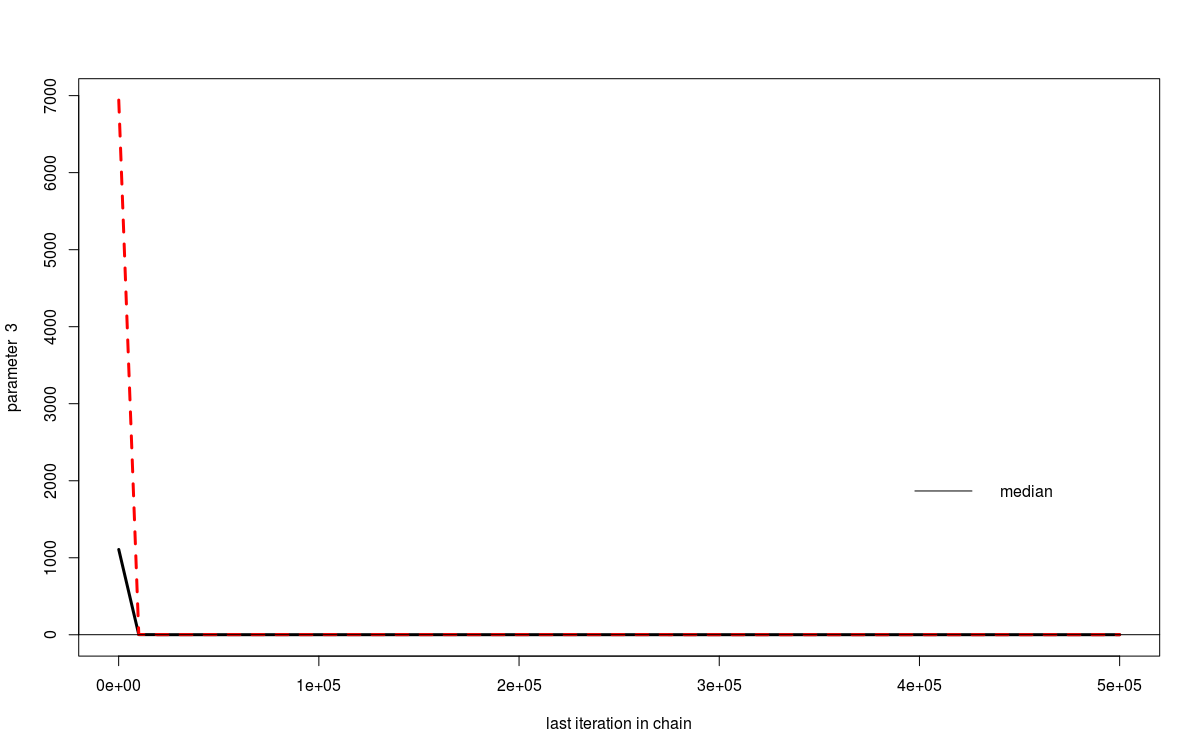
\includegraphics[scale=0.2]{scale_red_par3.png}
\caption{}
\label{}
\end{subfigure}
\begin{subfigure}{.5\textwidth}
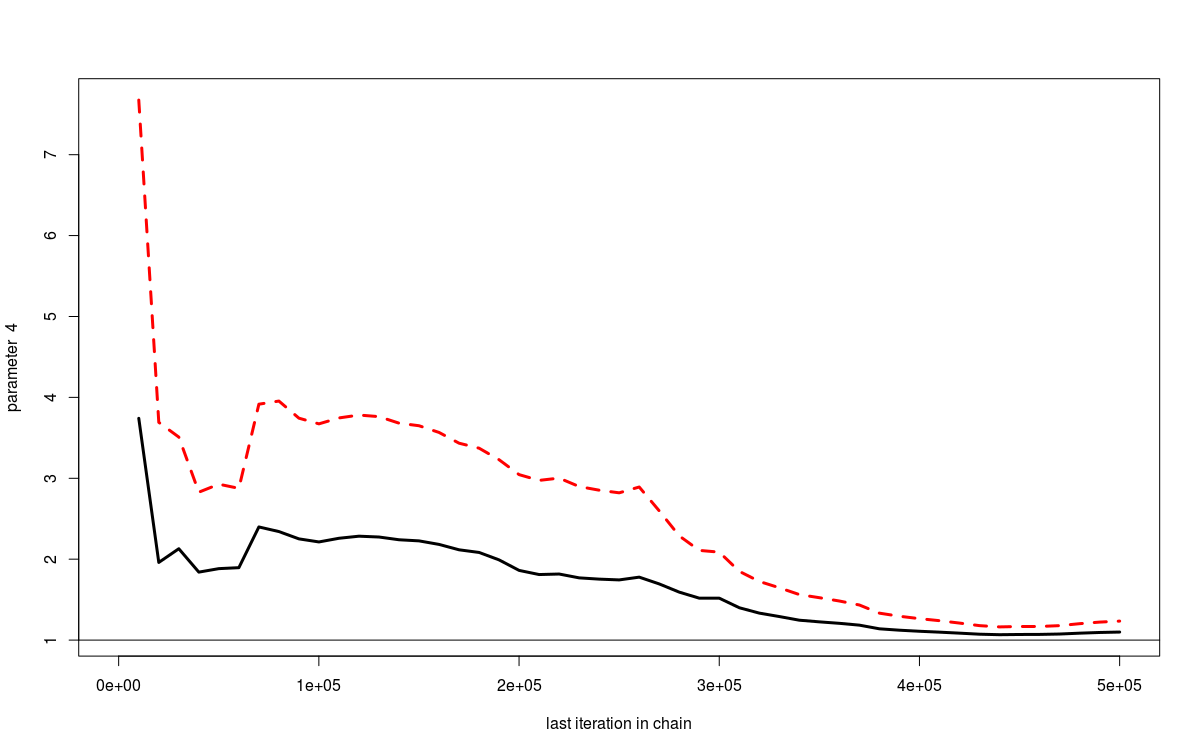
\includegraphics[scale=0.2]{scale_red_par4.png}
\caption{}
\label{}
\end{subfigure}
\caption{}
\label{Gelman-Rubin convergence plot}
\end{figure}

\begin{figure}[ht]
\centerline{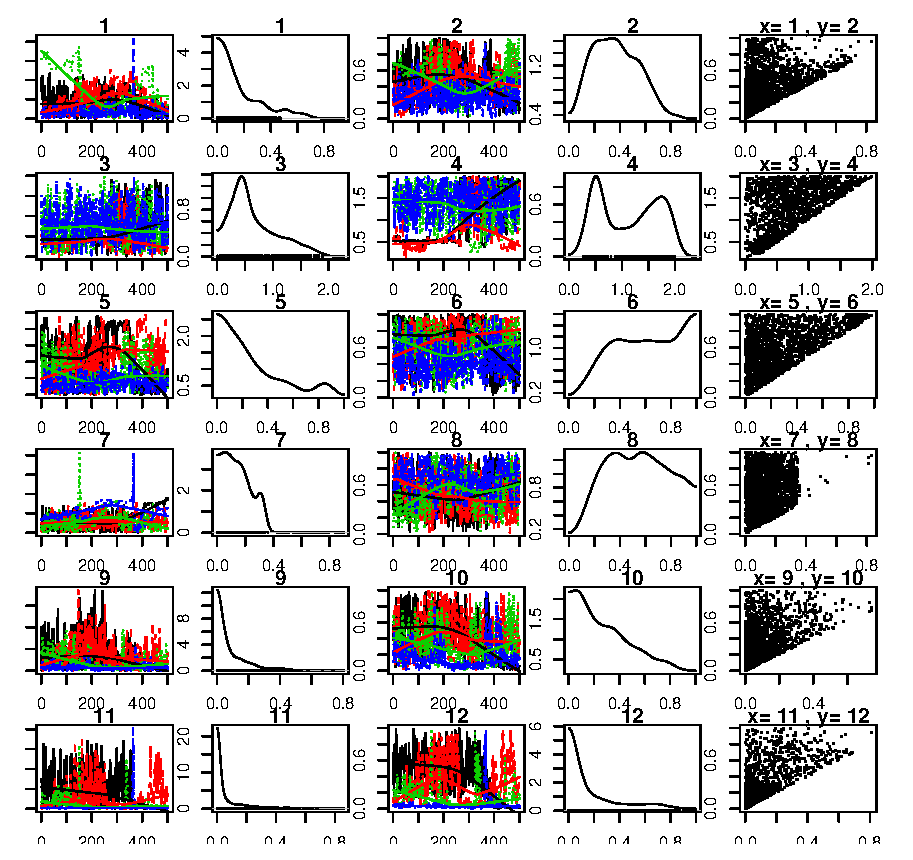
\includegraphics[]{distr-par1-12.eps}}
\caption{} 
\label{}
\end{figure}
\begin{figure}[ht]
\centerline{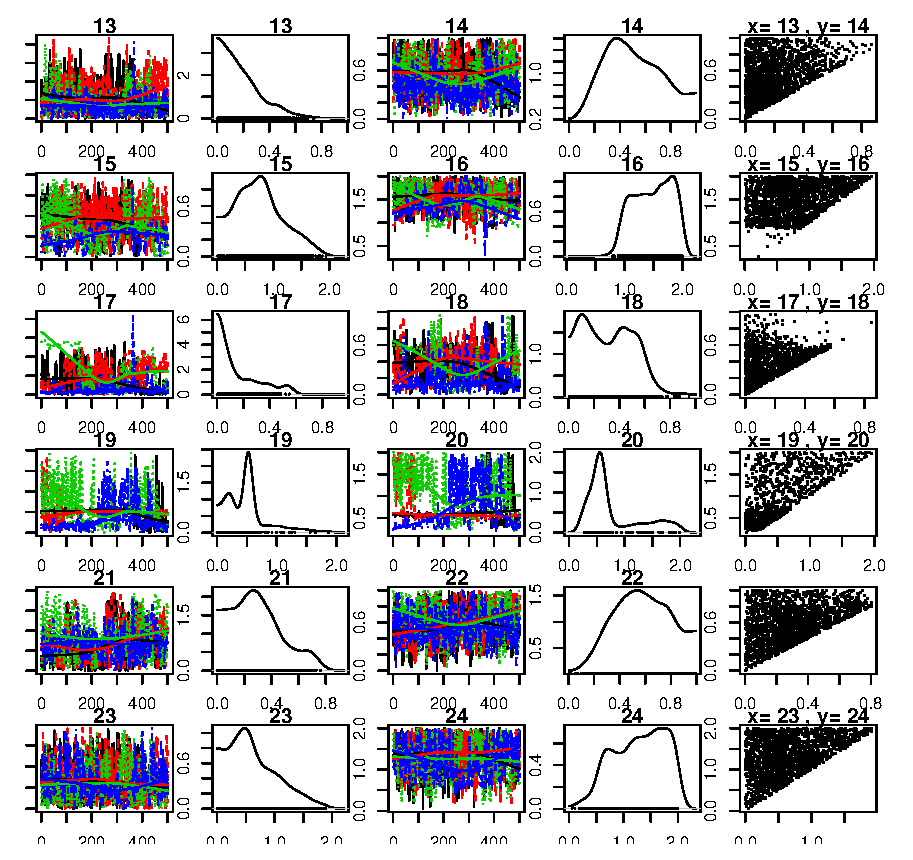
\includegraphics[]{distr-par13-24.eps}}
\caption{Still need to add a caption} 
\label{fig: parameter summary}
\end{figure}



%%% End document
\end{document}